\documentclass[11pt]{amsart}
\usepackage{geometry}                % See geometry.pdf to learn the layout options. There are lots.
\geometry{letterpaper}                   % ... or a4paper or a5paper or ... 
%\geometry{landscape}                % Activate for for rotated page geometry
\usepackage[parfill]{parskip}    % Activate to begin paragraphs with an empty line rather than an indent
\usepackage{graphicx}
\usepackage{amssymb}
\usepackage{epstopdf}
\DeclareGraphicsRule{.tif}{png}{.png}{`convert #1 `dirname #1`/`basename #1 .tif`.png}
\usepackage{listings}
\usepackage{xcolor}
\usepackage{hyperref}


\title{An Exploration of Atlanta Neighborhood Boundaries using KNN Classifiers}
\author{Katie Fullerton}
%\date{}                                           % Activate to display a given date or no date

\begin{document}
\lstset{    string=[s]{"}{"},
    stringstyle=\color{blue},
    comment=[l]{:},
    commentstyle=\color{black}
}
\maketitle
%------------------------------------------------------------------------------------------------
\section{Introduction}
%--------------------------------------------
\subsection{Background}
Atlanta is a major city in the south-eastern portion of the United States originally founded at the intersection of multiple railroad lines. As a city it has grown extensively in the last 50 years. Much of the planning efforts for that growth have been left to commercial developers, and consequently the city is somewhat a jumble of neighborhoods. Residents often complain that neighborhood boundaries are poorly-defined and have little connection with the actual usage patterns of the space. 
The city of Atlanta is divided into a number of Neighborhood Planning Units (NPUs). Each NPU is administered by a citizen and city employee council. These councils are empowered in various ways across the city, and have varying degrees of neighborhood buy-in. However, most NPUs do exert influence in the city zoning office, and thus can effect the type of development allowed within their borders. 
%--------------------------------------------
\subsection{Problem}
This system of NPUs was designed in the late 1970's. The past 50 years have seen dramatic shifts in population density, usage, and demographics in the Atlanta area. The purpose of this project is to compare the NPU boundaries designed in the 1970's to actual location usage patterns and determine if those boundaries still represent meaningful delineations.
This analysis would be of use to the city's planning board. If NPUs truly reflected the ways that citizens use their space, they would be more likely to get involved in the administration of those neighborhoods. Increased civic engagement has benefits both for the citizens and the city. This data might offer commercial value to developers looking to appeal to a specific consumer type, or to place new developments in areas of high likely usage.  
%------------------------------------------------------------------------------------------------
\section{Data}
%--------------------------------------------
\subsection{Data Sources}
In order to perform the analysis, we will need two separate data sets. The first required data set is the geospatial boundary data for each NPU, as designed in the 1970's. The second required data set must capture current usage patterns of the spaces in those geospatial regions. For the first dataset, we will access the City of Atlanta's GIS System via their website. The second dataset will be collected through the Foursquare API. It is assumed that Foursquare data represents real-time, up to date information about the way people live, work, and play in their neighborhoods.
\subsubsection{Geospatial Data}
The City of Atlanta offers a useful API explorer at \url{https://dcp-coaplangis.opendata.arcgis.com/datasets/npu/geoservice} . The resulting json file contains the information below. The fields of interest for this investigation are the NAME and geometry fields. 

\begin{lstlisting}
 { "attributes": {
            "OBJECTID": 260,
            "LOCALID": null,
            "NAME": "K",
            "GEOTYPE": "NPU",
            "FULLFIPS": null,
            "LEGALAREA": null,
            "ACRES": 1528.29,
            "SQMILES": 2.39,
            "OLDNAME": null,
            "NPU": null
         },
         "geometry": {
            "rings": [
               [
                  [
                     -84.4173772073577,
                     33.772197013770004
                  ],
\end{lstlisting}

Using this tool, we generated a request URL \url{https://gis.atlantaga.gov/dpcd/rest/services/OpenDataService/FeatureServer/4/query?where=1%3D1&outFields=NAME&outSR=4326&f=json} to create a simplified output object with only the fields of interest. 
\subsubsection{Location Usage Data}
In order to collect a sufficient amount of data for the large geographical area covered, we created a latitude and longitude search grid. This grid was set to contain 10 steps between the minimum and maximum latitude and longitude values present in the GIS data. The resulting search grid can be seen in Figure \ref{fig:gridmap}. For each coordinate in Figure \ref{fig:gridmap}, a url was generated to query the Foursquare API. An anonymized sample URL is: \url{https://api.foursquare.com/v2/venues/explore?client_id=XXXXXXXX&client_secret=XXXXXXX&ll=33.886869733912235,-84.28962468321286&v=20180604&limit=50&radius=4500}.
The results of each API call were compiled into a single large dataframe for cleaning.
\begin{figure}
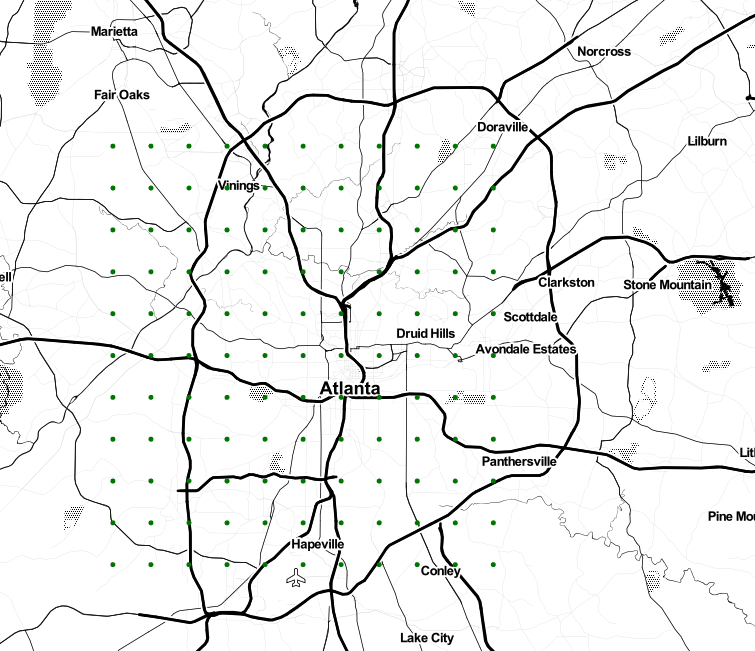
\includegraphics[width=\textwidth]{gridmap}
\caption{Latitude and Longitude Search Grid}
\label{fig:gridmap}
\end{figure}
%--------------------------------------------
\subsection{Data Cleaning}
\subsubsection{Cleaning Geospatial Data}

\subsubsection{Cleaning Location Usage Data}
Once retrieved, the location usage data contains significantly more data than needed for this analysis. The initial output format can be seen in Table \ref{tab:fsraw}

\begin{figure}
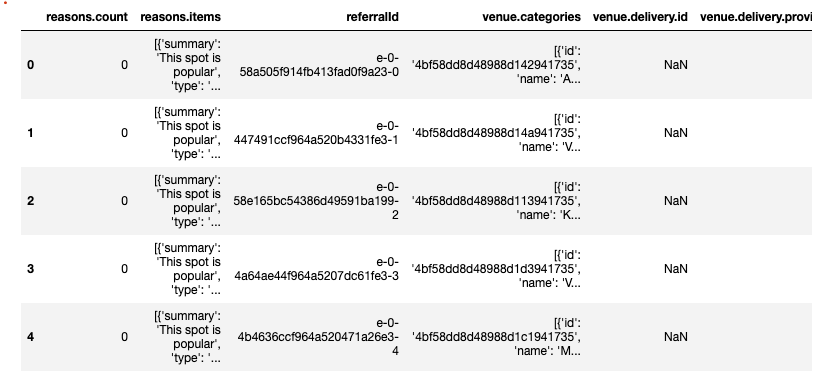
\includegraphics[width=0.8\textwidth]{Foursquare_API_output_table_raw}
\caption{Raw data output from Foursquare}
\label{tab:fsraw}
\end{figure}

The name, latitude, and longitude attributes could be directly extracted. The category field contained additional structure, so a function was written to extract the category string from that structure, as shown below. 
Initially, it appeared that the Foursquare data did include a neighborhood categorization. However, as the analysis continued, it became apparent that this field is either 'NaN' or left out of the data set entirely. While processing, a conditional clause was created, as seen below, to facilitate the compilation of the data.  In the final model, this data was determined to offer no additional value to the analysis. 

\lstset{language=Python}
\begin{lstlisting}[caption={Category Extraction Function}]
def get_category_type(row):
    try:
        categories_list = row['categories']
    except:
        categories_list = row['venue.categories']
        
    if len(categories_list) == 0:
        return None
    else:
        return categories_list[0]['name']
\end{lstlisting}

\begin{lstlisting}[caption={Neighborhood Data Screening Clause}]
 if 'venue.location.neighborhood' in list(dataframe.columns.values):
        data['neighborhood'] = dataframe['venue.location.neighborhood']
    else: 
        data['neighborhood'] = np.nan
        
\end{lstlisting}
\begin{figure}
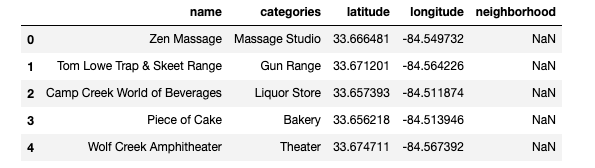
\includegraphics[width=0.8\textwidth]{Foursquare_API_output_table_cleaned}
\caption{Cleaned Location Dataframe}
\label{tab:fsclean}
\end{figure}

The search grid was constructed orthogonally, while the Foursquare interface assumes a circular search radius. Consequently, there are likely to be a number of locations that are captured in more than on API call. Duplicate data does not provide additional information for this analysis, and so duplicates were removed. The initial search resulted in 5970 total location listings, with only 1913 unique values. It was determined that this is a sufficient number for training and testing of a model. However, correcting the discrepancy between square and circular searches could increase the number of unique data points for future work. 
%--------------------------------------------
\subsection{Exploratory Data Analysis}
\subsubsection{NPU Boundaries}
The NPU boundaries were described by a series of coordinates for each boundary. 
\begin{figure}
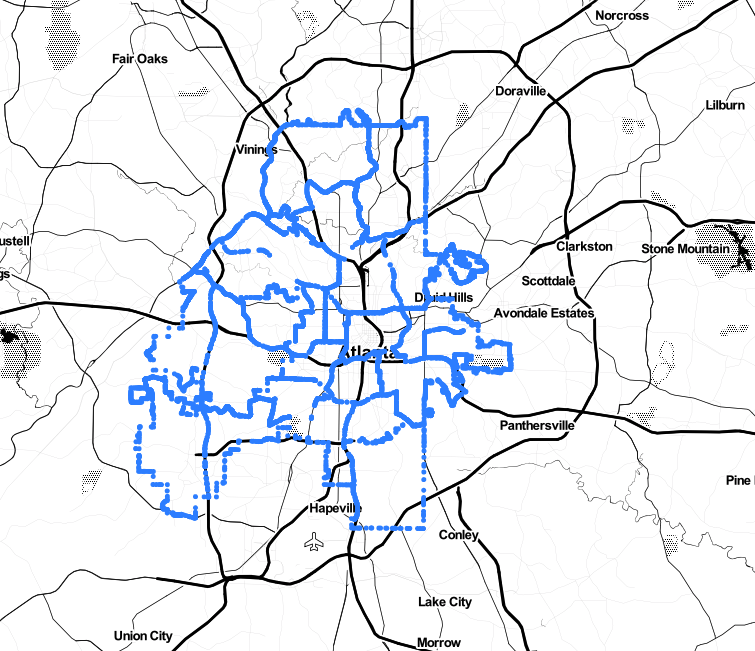
\includegraphics[width=\textwidth]{NPUoutlines.png}
\caption{NPU Boundaries in the City of Atlanta}
\label{fig:npuoutlines}
\end{figure}
\subsubsection{Foursquare Venue Data}
\begin{figure}
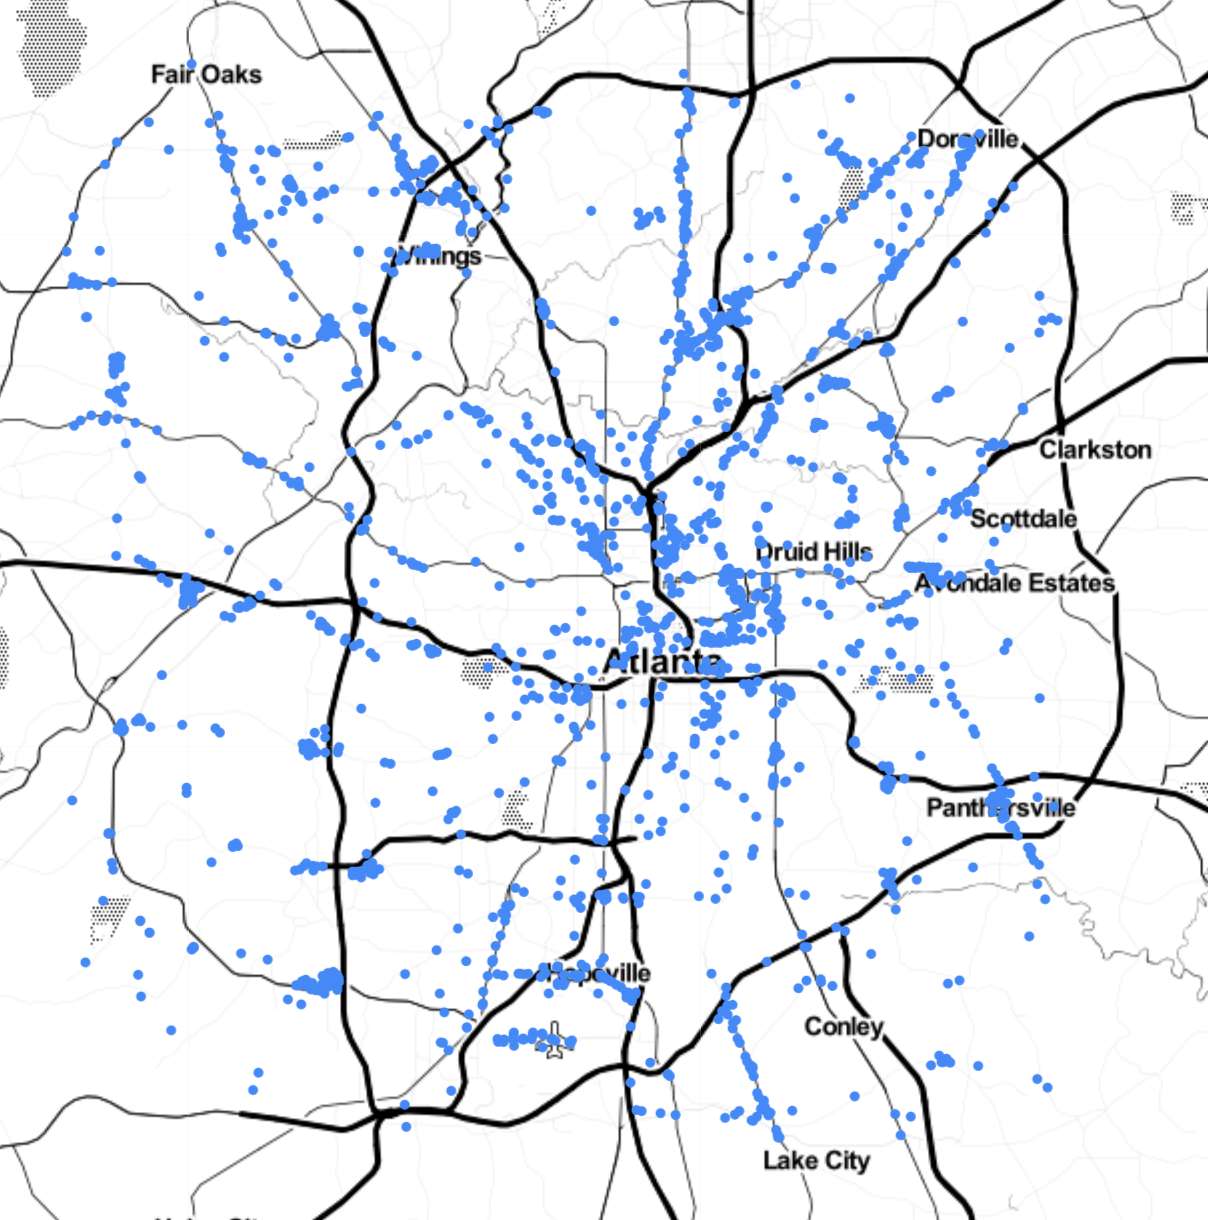
\includegraphics[width=\textwidth]{VenuesMap}
\caption{Results of Foursquare API call}
\label{fig:venues}
\end{figure}
%------------------------------------------------------------------------------------------------
\section{Methodology}
%--------------------------------------------
\subsection{NPU Assignment}
%--------------------------------------------
\subsection{KNN Classifier Construction}
%--------------------------------------------
\subsection{Cross Validation}
%------------------------------------------------------------------------------------------------
\section{Results}
%--------------------------------------------
\subsection{Scoring}
%--------------------------------------------
\subsection{Visual Analysis}
%------------------------------------------------------------------------------------------------
\section{Discussion}
%------------------------------------------------------------------------------------------------
\section{Conclusion}
%--------------------------------------------
\subsection{Future Work}


%------------------------------------------------------------------------------------------------
\end{document}  